\documentclass{article}
\usepackage[english]{babel}
\usepackage{graphicx}
\usepackage{graphicx,scalerel}
\begin{document}

\section*{Task 2:}

\subsection*{2a)}

mean = 33.55274553571429 \newline
standard deviation  = 78.87550070784701

\subsection*{2b)}
See code for implementation.
\subsection*{2c)}

\begin{figure}[h!]
    \centering
    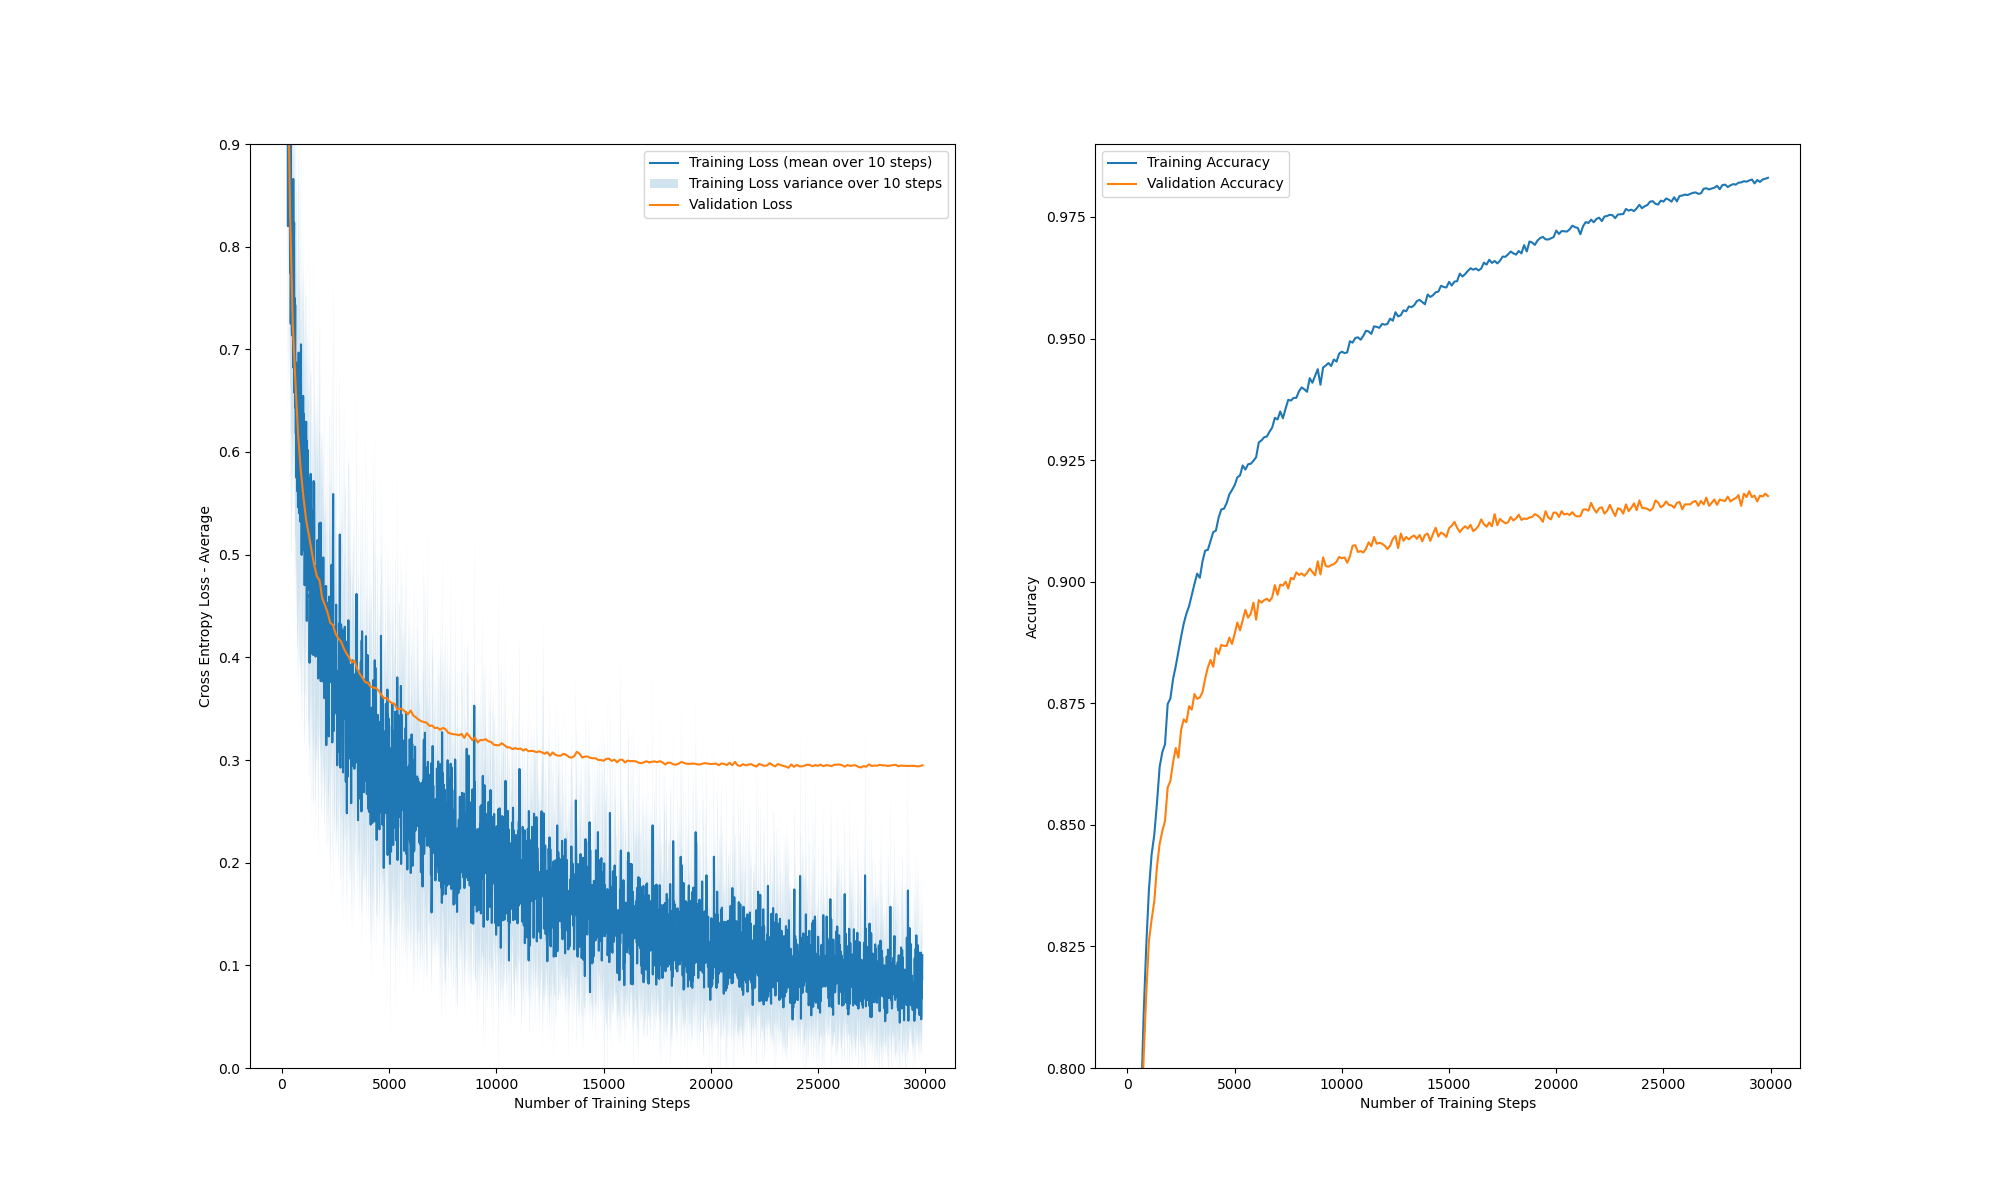
\includegraphics[width=\linewidth]{task2c_train_loss.png}
    \caption[short]{Plot of the training and validation loss and accuracy over training.}
\end{figure}


\subsection*{2d)}

We have an input layer with the size of 784. In addition we have 1 bias unit. The hidden layer will
get input from 785 nodes. Further, it has 64 nodes, which means there are 64 weights. We will 
get 785 * 64 parameters in this layer. In the next layer we have 10 nodes and it gets input from 64 nodes. This 64 *10 parameters.
In total we will have : \newline
\begin{equation}
    Number of parameters = 785 \cdot 64 + 64 \cdot 10 = 50880 
\end{equation}


\section*{Task 3 :}

\subsection*{3a)}
See code for implementation.
\subsection*{3b)}
See code for implementation.
\subsection*{3c)}
See code for implementation.






\section*{Task 4 : }

\subsection*{4a)}


\subsection*{4b)}

\subsection*{4c)}

\subsection*{4d)}
    
\subsection*{4e)}

\subsection*{4f)}


\end{document}